\documentclass[journal,compsoc, 10pt, draftclsnofoot, onecolumn]{IEEEtran}

\usepackage{graphicx}
\usepackage{amssymb}
\usepackage{amsmath}
\usepackage{amsthm}
\usepackage{tabularx}
\usepackage{graphicx}

\newcommand{\subparagraph}{}
\usepackage{titlesec}

\usepackage{alltt}
\usepackage{float}
\usepackage{color}
\usepackage{url}

\usepackage{balance}
\usepackage[TABBOTCAP, tight]{subfigure}
\usepackage{enumitem}
\usepackage{pstricks, pst-node}

\usepackage{cite}
\usepackage{listings}

\usepackage[margin=0.75in]{geometry}
\geometry{textheight=8.5in, textwidth=6in}

\renewcommand{\familydefault}{\sfdefault}


\newlength\tindent
\setlength{\tindent}{\parindent}
\setlength{\parindent}{0pt}
\renewcommand{\indent}{\hspace*{\tindent}}

\newcommand{\cred}[1]{{\color{red}#1}}
\newcommand{\cblue}[1]{{\color{blue}#1}}


\usepackage{hyperref}
\usepackage{geometry}

\lstset{
language=C,
basicstyle=\ttfamily,
commentstyle=\color{blue},
keywordstyle=\color{green},
numberstyle=\color{red},
stringstyle=\color{orange}
}

\def\nameD{Devin Foulger}
\def\nameH{Hector Trujillo}
\def\nameB{Bryan Liauw}

\usepackage{fancyvrb}
\usepackage{color}
\usepackage[latin1]{inputenc}


\makeatletter
\def\PY@reset{\let\PY@it=\relax \let\PY@bf=\relax%
    \let\PY@ul=\relax \let\PY@tc=\relax%
    \let\PY@bc=\relax \let\PY@ff=\relax}
\def\PY@tok#1{\csname PY@tok@#1\endcsname}
\def\PY@toks#1+{\ifx\relax#1\empty\else%
    \PY@tok{#1}\expandafter\PY@toks\fi}
\def\PY@do#1{\PY@bc{\PY@tc{\PY@ul{%
    \PY@it{\PY@bf{\PY@ff{#1}}}}}}}
\def\PY#1#2{\PY@reset\PY@toks#1+\relax+\PY@do{#2}}

\expandafter\def\csname PY@tok@gd\endcsname{\def\PY@tc##1{\textcolor[rgb]{0.63,0.00,0.00}{##1}}}
\expandafter\def\csname PY@tok@gu\endcsname{\let\PY@bf=\textbf\def\PY@tc##1{\textcolor[rgb]{0.50,0.00,0.50}{##1}}}
\expandafter\def\csname PY@tok@gt\endcsname{\def\PY@tc##1{\textcolor[rgb]{0.00,0.25,0.82}{##1}}}
\expandafter\def\csname PY@tok@gs\endcsname{\let\PY@bf=\textbf}
\expandafter\def\csname PY@tok@gr\endcsname{\def\PY@tc##1{\textcolor[rgb]{1.00,0.00,0.00}{##1}}}
\expandafter\def\csname PY@tok@cm\endcsname{\let\PY@it=\textit\def\PY@tc##1{\textcolor[rgb]{0.25,0.50,0.50}{##1}}}
\expandafter\def\csname PY@tok@vg\endcsname{\def\PY@tc##1{\textcolor[rgb]{0.10,0.09,0.49}{##1}}}
\expandafter\def\csname PY@tok@m\endcsname{\def\PY@tc##1{\textcolor[rgb]{0.40,0.40,0.40}{##1}}}
\expandafter\def\csname PY@tok@mh\endcsname{\def\PY@tc##1{\textcolor[rgb]{0.40,0.40,0.40}{##1}}}
\expandafter\def\csname PY@tok@go\endcsname{\def\PY@tc##1{\textcolor[rgb]{0.50,0.50,0.50}{##1}}}
\expandafter\def\csname PY@tok@ge\endcsname{\let\PY@it=\textit}
\expandafter\def\csname PY@tok@vc\endcsname{\def\PY@tc##1{\textcolor[rgb]{0.10,0.09,0.49}{##1}}}
\expandafter\def\csname PY@tok@il\endcsname{\def\PY@tc##1{\textcolor[rgb]{0.40,0.40,0.40}{##1}}}
\expandafter\def\csname PY@tok@cs\endcsname{\let\PY@it=\textit\def\PY@tc##1{\textcolor[rgb]{0.25,0.50,0.50}{##1}}}
\expandafter\def\csname PY@tok@cp\endcsname{\def\PY@tc##1{\textcolor[rgb]{0.74,0.48,0.00}{##1}}}
\expandafter\def\csname PY@tok@gi\endcsname{\def\PY@tc##1{\textcolor[rgb]{0.00,0.63,0.00}{##1}}}
\expandafter\def\csname PY@tok@gh\endcsname{\let\PY@bf=\textbf\def\PY@tc##1{\textcolor[rgb]{0.00,0.00,0.50}{##1}}}
\expandafter\def\csname PY@tok@ni\endcsname{\let\PY@bf=\textbf\def\PY@tc##1{\textcolor[rgb]{0.60,0.60,0.60}{##1}}}
\expandafter\def\csname PY@tok@nl\endcsname{\def\PY@tc##1{\textcolor[rgb]{0.63,0.63,0.00}{##1}}}
\expandafter\def\csname PY@tok@nn\endcsname{\let\PY@bf=\textbf\def\PY@tc##1{\textcolor[rgb]{0.00,0.00,1.00}{##1}}}
\expandafter\def\csname PY@tok@no\endcsname{\def\PY@tc##1{\textcolor[rgb]{0.53,0.00,0.00}{##1}}}
\expandafter\def\csname PY@tok@na\endcsname{\def\PY@tc##1{\textcolor[rgb]{0.49,0.56,0.16}{##1}}}
\expandafter\def\csname PY@tok@nb\endcsname{\def\PY@tc##1{\textcolor[rgb]{0.00,0.50,0.00}{##1}}}
\expandafter\def\csname PY@tok@nc\endcsname{\let\PY@bf=\textbf\def\PY@tc##1{\textcolor[rgb]{0.00,0.00,1.00}{##1}}}
\expandafter\def\csname PY@tok@nd\endcsname{\def\PY@tc##1{\textcolor[rgb]{0.67,0.13,1.00}{##1}}}
\expandafter\def\csname PY@tok@ne\endcsname{\let\PY@bf=\textbf\def\PY@tc##1{\textcolor[rgb]{0.82,0.25,0.23}{##1}}}
\expandafter\def\csname PY@tok@nf\endcsname{\def\PY@tc##1{\textcolor[rgb]{0.00,0.00,1.00}{##1}}}
\expandafter\def\csname PY@tok@si\endcsname{\let\PY@bf=\textbf\def\PY@tc##1{\textcolor[rgb]{0.73,0.40,0.53}{##1}}}
\expandafter\def\csname PY@tok@s2\endcsname{\def\PY@tc##1{\textcolor[rgb]{0.73,0.13,0.13}{##1}}}
\expandafter\def\csname PY@tok@vi\endcsname{\def\PY@tc##1{\textcolor[rgb]{0.10,0.09,0.49}{##1}}}
\expandafter\def\csname PY@tok@nt\endcsname{\let\PY@bf=\textbf\def\PY@tc##1{\textcolor[rgb]{0.00,0.50,0.00}{##1}}}
\expandafter\def\csname PY@tok@nv\endcsname{\def\PY@tc##1{\textcolor[rgb]{0.10,0.09,0.49}{##1}}}
\expandafter\def\csname PY@tok@s1\endcsname{\def\PY@tc##1{\textcolor[rgb]{0.73,0.13,0.13}{##1}}}
\expandafter\def\csname PY@tok@sh\endcsname{\def\PY@tc##1{\textcolor[rgb]{0.73,0.13,0.13}{##1}}}
\expandafter\def\csname PY@tok@sc\endcsname{\def\PY@tc##1{\textcolor[rgb]{0.73,0.13,0.13}{##1}}}
\expandafter\def\csname PY@tok@sx\endcsname{\def\PY@tc##1{\textcolor[rgb]{0.00,0.50,0.00}{##1}}}
\expandafter\def\csname PY@tok@bp\endcsname{\def\PY@tc##1{\textcolor[rgb]{0.00,0.50,0.00}{##1}}}
\expandafter\def\csname PY@tok@c1\endcsname{\let\PY@it=\textit\def\PY@tc##1{\textcolor[rgb]{0.25,0.50,0.50}{##1}}}
\expandafter\def\csname PY@tok@kc\endcsname{\let\PY@bf=\textbf\def\PY@tc##1{\textcolor[rgb]{0.00,0.50,0.00}{##1}}}
\expandafter\def\csname PY@tok@c\endcsname{\let\PY@it=\textit\def\PY@tc##1{\textcolor[rgb]{0.25,0.50,0.50}{##1}}}
\expandafter\def\csname PY@tok@mf\endcsname{\def\PY@tc##1{\textcolor[rgb]{0.40,0.40,0.40}{##1}}}
\expandafter\def\csname PY@tok@err\endcsname{\def\PY@bc##1{\setlength{\fboxsep}{0pt}\fcolorbox[rgb]{1.00,0.00,0.00}{1,1,1}{\strut ##1}}}
\expandafter\def\csname PY@tok@kd\endcsname{\let\PY@bf=\textbf\def\PY@tc##1{\textcolor[rgb]{0.00,0.50,0.00}{##1}}}
\expandafter\def\csname PY@tok@ss\endcsname{\def\PY@tc##1{\textcolor[rgb]{0.10,0.09,0.49}{##1}}}
\expandafter\def\csname PY@tok@sr\endcsname{\def\PY@tc##1{\textcolor[rgb]{0.73,0.40,0.53}{##1}}}
\expandafter\def\csname PY@tok@mo\endcsname{\def\PY@tc##1{\textcolor[rgb]{0.40,0.40,0.40}{##1}}}
\expandafter\def\csname PY@tok@kn\endcsname{\let\PY@bf=\textbf\def\PY@tc##1{\textcolor[rgb]{0.00,0.50,0.00}{##1}}}
\expandafter\def\csname PY@tok@mi\endcsname{\def\PY@tc##1{\textcolor[rgb]{0.40,0.40,0.40}{##1}}}
\expandafter\def\csname PY@tok@gp\endcsname{\let\PY@bf=\textbf\def\PY@tc##1{\textcolor[rgb]{0.00,0.00,0.50}{##1}}}
\expandafter\def\csname PY@tok@o\endcsname{\def\PY@tc##1{\textcolor[rgb]{0.40,0.40,0.40}{##1}}}
\expandafter\def\csname PY@tok@kr\endcsname{\let\PY@bf=\textbf\def\PY@tc##1{\textcolor[rgb]{0.00,0.50,0.00}{##1}}}
\expandafter\def\csname PY@tok@s\endcsname{\def\PY@tc##1{\textcolor[rgb]{0.73,0.13,0.13}{##1}}}
\expandafter\def\csname PY@tok@kp\endcsname{\def\PY@tc##1{\textcolor[rgb]{0.00,0.50,0.00}{##1}}}
\expandafter\def\csname PY@tok@w\endcsname{\def\PY@tc##1{\textcolor[rgb]{0.73,0.73,0.73}{##1}}}
\expandafter\def\csname PY@tok@kt\endcsname{\def\PY@tc##1{\textcolor[rgb]{0.69,0.00,0.25}{##1}}}
\expandafter\def\csname PY@tok@ow\endcsname{\let\PY@bf=\textbf\def\PY@tc##1{\textcolor[rgb]{0.67,0.13,1.00}{##1}}}
\expandafter\def\csname PY@tok@sb\endcsname{\def\PY@tc##1{\textcolor[rgb]{0.73,0.13,0.13}{##1}}}
\expandafter\def\csname PY@tok@k\endcsname{\let\PY@bf=\textbf\def\PY@tc##1{\textcolor[rgb]{0.00,0.50,0.00}{##1}}}
\expandafter\def\csname PY@tok@se\endcsname{\let\PY@bf=\textbf\def\PY@tc##1{\textcolor[rgb]{0.73,0.40,0.13}{##1}}}
\expandafter\def\csname PY@tok@sd\endcsname{\let\PY@it=\textit\def\PY@tc##1{\textcolor[rgb]{0.73,0.13,0.13}{##1}}}

\def\PYZbs{\char`\\}
\def\PYZus{\char`\_}
\def\PYZob{\char`\{}
\def\PYZcb{\char`\}}
\def\PYZca{\char`\^}
\def\PYZam{\char`\&}
\def\PYZlt{\char`\<}
\def\PYZgt{\char`\>}
\def\PYZsh{\char`\#}
\def\PYZpc{\char`\%}
\def\PYZdl{\char`\$}
\def\PYZti{\char`\~}
% for compatibility with earlier versions
\def\PYZat{@}
\def\PYZlb{[}
\def\PYZrb{]}
\makeatother


\hypersetup {
        colorlinks = true,
        urlcolor = black,
        linkcolor = black,
        pdfauthor = {\nameD\nameH\nameB},
        pdfkeywords = {},
        pdfsubject = {},
        pdfpagemode = UseNone
}

\titleformat{\section}
	{\normalfont\fontsize{15}{10}\bfseries}{\thesection}{1em}{}
\titleformat{\subsection}
	{\normalfont\fontsize{12}{15}\bfseries}{\thesubsection}{1em}{}
\titleformat{\subsubsection}
	{\normalfont\fontsize{12}{15}\bfseries}{\thesubsubsection}{1em}{}

\begin{document}

\title{\vspace{20em}Software Rquirements Specification \\{\vspace{-1ex}\huge College Merchandise} \\ {\large \today}}
\author{\vspace{10ex}Devin Foulger \\{\vspace{-1ex}Hector Trujillo} \\{\vspace{-1ex}Bryan Liauw}}

\begin{titlepage}

\maketitle
\thispagestyle{empty}

\end{titlepage}

\tableofcontents

\section{INTRODUCTION}

This section will provide an overview of what is included in this Software 
Requirements Document (SRS).

\subsection{Purpose}

This SRS document will serve several purposes. First it will define the 
requirements for the "College Merchandising" application that team 
"DHB Solutions" will be developing for their CS Capstone project for eBay. The 
document will detailing the constraints, features, dependencies and performance 
of the application in a manner that clearly demonstrates what the client will be
 receiving.The intended audience for this Software Requirements Specification 
(SRS) will be the team, eBay, and the instructors of the computer science senior
 capstone class at Oregon State University. 

\subsection{Scope}

The Android Application "College Merchandising" will allow users to browse and 
shop for college merchandise that are for sale through eBay. The application 
will be published to the Google Play Store and will be optimized for Android's 
latest operating system 'N'. \newline

This application will also demonstrate the use and functionality of eBay's 
public APIs by allowing users to search eBay's inventory of items. The 
application will allow users to filter out their search results by different 
criteria. The application will also allow users to purchase items from eBay. 

\subsection{Definitions, acronums, and abbreviations}

Below are definitions for terms that will allow for proper interpretation of the
 requirements document.

\begin{table}[]
\centering
\caption{Definitions}
\label{my-label}
\begin{tabularx}{\textwidth}{X|X}
\hline
\textbf{Term}               & \textbf{Definition}                                                                                                           \\ \hline
API                    	      & Application Programming Interface, allows developers to develop applications that connect to eBay's large inventory of items. \\ \hline
Shop                   	      & Search for and view college related items on sale through eBay.                                                               \\ \hline
Vendors               	      & Individuals or companies that sell or will sell items on eBay                                                                 \\ \hline
Filters                	      & Search criteria that will allow the user to more easily find the item that they are looking for.                              \\ \hline
Third-Party Developers & Individuals outside of eBay that will be using eBay's public APIs to create their own applications.                           \\ \hline
Application            	      & An Android application that uses eBay's public APIs.                                                                          \\ \hline
Interface              	      & The User Interface.                                                                                                           \\ \hline
Bugs                   	      & Errors in the API code that may be discovered during use.                                                                     \\ \hline
College Merchandise     & Items such as school supplies for Higher Ed, fan gear, etc...                                                                 \\ \hline
User                   	      & Any one who will be using the Android Application utilizing eBay's APIs.                                                      \\ \hline
Client                 	      & eBay                                                                                                                          \\ \hline
BIN                    	      & Buy It Now                                                                                                                    \\ \hline
N                   	      & Android's new Nougat operating system 
\\ \hline
M                   	      & Android's Marshmallow operating system                                                                                                                   \\ \hline
\end{tabularx}
\end{table}

\newpage

\subsection{Overview}

The remainder of this document will provide an overview of the functionality 
that the "College Merchandising" application will offer along with the 
interaction that it will have with other systems. The next chapter will identify
 any constraints that may prevent success for this project.

\section{OVERALL DESCRIPTION}

This section will provide the reader with an overview of the entire application.
 The application will be explained in a way that the functionality is easily 
identified along with any constraints.

\subsection{Product Perspective}

The android application will communicate with eBay to provide the user with the 
opportunity to shop through their inventory of college related merchandise. The 
communication will be accomplished with the use of eBay's APIs. This 
communication is important to provide the user with a seamless shopping 
experience without having to switch between different applications.\newline

Since no data regarding the inventory of items that eBay provides will be stored
 by this application, there will be a constant need for an Internet connection 
to be able to pull search results from eBay's inventory. 

\subsubsection{User Interfaces}

The user interface will mimic what people already know about eBay and other 
similar shopping experiences. This will include standard things such as a place 
to sign in, a place to search for items, and a place to view items. Signing in 
could consist of multiple pages for existing users or for new users. Searching 
could also vary depending on search settings like a basic search or advanced 
searching. When viewing items, there could be several kinds of list views. We 
would also have specific college-related images to help users to find the item 
that they are looking for. Since our application is limited to college 
merchandises, we will have some visual appeals that reflect what the application
 is about.

\subsubsection{Hardware Interfaces}

The devices that we use must be compatible with M and N os. 

\subsubsection{Software Interfaces}

We will be using the new Android operating system, N. We will also be making use
 of a wide variety of eBay's new APIs. Some of these are apart of their new Buy 
APIs. These ones include the Browse and Order APIs. The Browse API will allow us
 to search for items and find different item feeds. The Order API will allow us 
to have some form of item checkout and order tracking. Will we also make use of 
their Finding API, which will allow us to search for items. Together, these APIs
 will allow us to connect with eBay's large collection of items.

\subsubsection{Communication Interfaces}

The device should always have some form of connection to the internet. This 
means the device can connect in one of two ways. The first being through the 
devices WLAN. The second being that it could connect using its cellular data.

\subsubsection{Operations}

There will be many user initiated operations. These include searching and 
purchasing. Searching means that the user will be finding items with specific 
search criteria. The items that they find could be related to different schools,
 or have specific colors. Purchasing means that the user is able to select an 
item that they want and pay for it.\newline

The application should only be in use when a user is actually using it. There 
are no periods of unattended use. The only time that might be considered as 
unattended use, is when the application is gathering and displaying search 
results to the user. 

\subsection{Production Functions}

There are a couple of major features that this application will support. It will
 allow for users to search for items and to purchase them. Users will be able 
to browse eBay's large collection of college merchandise that they have for 
sale. The application will allow users to narrow down what they are looking for 
by allowing them to use filters such as types of items, condition, cost, college
 specific, by terms, and so on. \newline

The results of these searches will be displayed in either a listview that simply
 provides minor details regarding the item or thumbnail views that provide an 
image of the product along with a few details. The number of results displayed 
at once will vary depending on how the user wants the results presented to them 
and by the screen size of the product that they will be using. The application 
will also allow the user to sort the order in which the items are displayed. The
 sort options will be similar to what eBay provides on their current website. 
This includes sorting by price and time (ending soon or recently posted).

\subsection{User Characteristics}

Users will include individuals who are looking to find great deals on college 
merchandise online. The typical user will be someone who is looking for college 
merchandise. The actual user group could range between many different people. 
The main audience should be individuals looking for college merchandise and 
could be incoming college students, or people who are already college students. 
Users could also be parents, grandparents or other individuals who are looking 
to help out a relative or friend in searching for any college merchandise that 
the individual might need. \newline

Since are users are going to use this application on  a mobile device, 
our main focus to the user would be to create an interface that is simple
 and straightforward. The user should be able to learn and familiarize with the interface
 in a short period of time. Furthermore, the processes should be fast; the 
window between processes should be short to keep the attention of the users.

\subsection{Constraints}

Android's new operating system, N OS, will be the biggest constraint. This is 
because the operating system is new and is not present on many of today's top 
Android devices. This also means that the documentation may not be up to date 
with the new operating system. Older APIs created by Google may also be
 deprecated.\newline

Large loads on the application might put strain on lower quality machines. 
Example of large loads would be a lot of activities and threads and overly 
large image.Testing might also be a constraint since a virtual machine will take a huge 
amount of computer resources. For a better testing environment, the usage of an 
actual physical smartphone might be needed.

\subsection{Assumptions and Dependancies}

An assumption and dependency for this project will be the availability of the 
Android operating system N and a device that can run it. A secondary assumption 
is that the mobile phone which the application will be running on will have an 
active internet connection. A third assumption would be that users of the 
application will have an eBay account that they will be able to use to save 
searched items and even checkout and complete a purchase through the 
application. A dependency that the application will have is that we highly 
depends on the connection to the Ebay database. If the database server is down, 
we might not get the app to work.

\section{SPECIFIC REQUIREMENTS}

\subsection{Functional Requirements}

This section defines all the requirements that are fundamental actions to the 
application.

\subsubsection{Functional Requirement 1}
Name: Download application \newline
Description: The user must be able to download the application from the Google 
Play store. \newline
Input: None. \newline
Output: Application will be installed on the user's device. \newline
Dependencies: The user has an Android device that can support N os.

\subsubsection{Functional Requirement 2}
Name: Update application\newline
Description: This should allow the user to update the application via the Google
 Play store.\newline
Input: None.\newline
Output: Update application.\newline
Dependencies: The user has an Android device that can support N os.

\subsubsection{Functional Requirement 3}
Name: Sign in\newline
Description: This should allow the user to sign in to our application using and 
eBay account.\newline
Input: User's password and username for their eBay account.\newline
Output: Confirmation that user signed in.\newline
Dependencies: Functional requirement 1.

\subsubsection{Functional Requirement 4}
Name: Determine search criteria\newline
Description: The user should be able to select what they want to search for. The
 user should be able to select between many options. These include search by BIN
 (Buy It Now), price, school, color, condition, and bidding. They should also be
 able to use different search criteria in combination.\newline
Input: A combination of the above stated search criteria.\newline
Output: None.\newline
Dependencies: Functional requirement 1.

\subsubsection{Functional Requirement 5}
Name: Search by BIN\newline
Description: Allow the user to search by items tagged as BIN (Buy It Now).
\newline
Input: Allow the user to select BIN as a search option.\newline
Output: Search displays that the items displayed are only BIN items.\newline
Dependencies: Functional requirement 4.

\subsubsection{Functional Requirement 6}
Name: Search by price\newline
Description: The user should be able determine a price range in which their 
item should cost. There should be a minimum and maximum price. \newline
Input: A minimum price, a maximum price, or both.\newline
Output: None.\newline
Dependencies: Functional requirement 4.

\subsubsection{Functional Requirement 7}
Name: Search by school\newline
Description: The user should be able to search for a specific school or select 
from a pre-determined list of schools.\newline
Input: The specific school the user is searching for.\newline
Output: None.\newline
Dependencies: Functional requirement 4.

\subsubsection{Functional Requirement 8}
Name: Search by condition\newline
Description: The user should be able to search for items ranging from very used 
to new.\newline
Input: The condition of the item the user is searching for.\newline
Output: None.\newline
Dependencies: Functional requirement 4.

\subsubsection{Functional Requirement 9}
Name: Purchase\newline
Description: The user should be able to purchase an item that they have searched
 for.\newline
Input: The item that is going to be purchased.\newline
Output: Some receipt or confirmation that the item has been ordered.\newline
Dependencies: Functional requirement 4.

\subsubsection{Functional Requirement 10}
Name: Display search results\newline
Description: Search results should be displayed to the user given the user's 
search criteria. Search results should also be displayed according to how the 
user specifies. That should be able to display results from lowest price to 
largest price, or from BIN to bid.\newline
Input: None.\newline
Output: A list of items organized the way the user has specified.\newline
Dependencies: Functional requirements 4.

\subsubsection{Functional Requirement 11}
Name: Display search results (no results found)\newline
Description: This should display a list that doesn't include any items and will 
have a simple message stating that no items could be found. \newline
Input: None.\newline
Output: A simple message that states nothing could be found.\newline
Dependencies: Functional requirement 4.

\subsubsection{Functional Requirement 12}
Name: Item view for a selected item\newline
Description: When a user selects an item, it should be displayed in its own view
 with greater detail.\newline
Input: Item from listview.\newline
Output: A page with complete detail of the item.\newline
Dependencies: Functional requirement 10.

\subsection{Performance Requirements}

This section will document that the requirements provide a measurement of how 
the application will perform.

\subsubsection{Performance Requirement 1}
Name: Search feature\newline
Measurement: The search feature should be easy to find and easy to use.\newline
Dependencies: None.

\subsubsection{Performance Requirement 2}
Name: Usage of search feature\newline
Measurement: The search criteria provided should be easy to understand and 
simple.\newline
Dependencies: Performance requirement 1.

\subsubsection{Performance Requirement 3}
Name: Usage of search results in a listview\newline
Measurement: The results displayed in a listview should provide the user with 
easy to understand results. Things like the item name, price, and school should 
be provided to the user.\newline
Dependencies: Performance requirement 1.

\subsubsection{Performance Requirement 4}
Name: Purchase feature\newline
Measurement: The purchase feature should mirror what users are already familiar 
to, such as a shopping cart with checkout buttons.\newline
Dependencies: None.

\subsubsection{Performance Requirement 5}
Name: Usage of purchase feature\newline
Measurement: Users should recieve a receipt that the feature worked.\newline 
Dependencies: Performance requirement 4.

\subsubsection{Performance Requirement 6}
Name: Sign in feature\newline
Measurement: The user should be able to find the sign in feature easily. They 
should also be able to sign in to their eBay accounts in a similar way to the 
online experience. \newline
Dependencies: None.

\subsubsection{Performance Requirement 7}
Name: Usage of sign in feature\newline
Measurement: The user should know that they are signed in. \newline
Dependencies: Performance requirement 6.

\subsection{Software System Attributes}

This section will define how are application will meet the software system 
attributes.

\subsubsection{Reliability}

The application should be able to search and purchase items according to what 
has been specified by the user.

\subsubsection{Availability}

The application will be available only to users who have Android devices. These 
users must also have devices that are compatible with the new operating system, 
N and the current operating system, M. Other than the two constraints above, 
any user who has a valid internet connection and access to the Google Play 
store, should be able to download and use our application.

\subsubsection{Security}

Security should not be a problem, as the APIs are using HTTPS protocols for 
recieving and sending data.

\subsubsection{Maintainabillity}

In order to create an application that is easily maintainable, we must be sure 
that all the parts are separated in an easy to manage fashion. We would avoid 
over-coupling objects and classes and use an MVC design pattern. Our code 
will also be testable, readable, and commented well.

\subsubsection{Portability}

We acknowledge the fact that our application will not be very portable. This is 
because we a specifically developing the application for Android systems. This 
means that our language is also going to be in Java. 

\newpage

\section{Appendices}
\subsection{Appendix I: Gannt Chart for Application}

\begin{figure}[h]
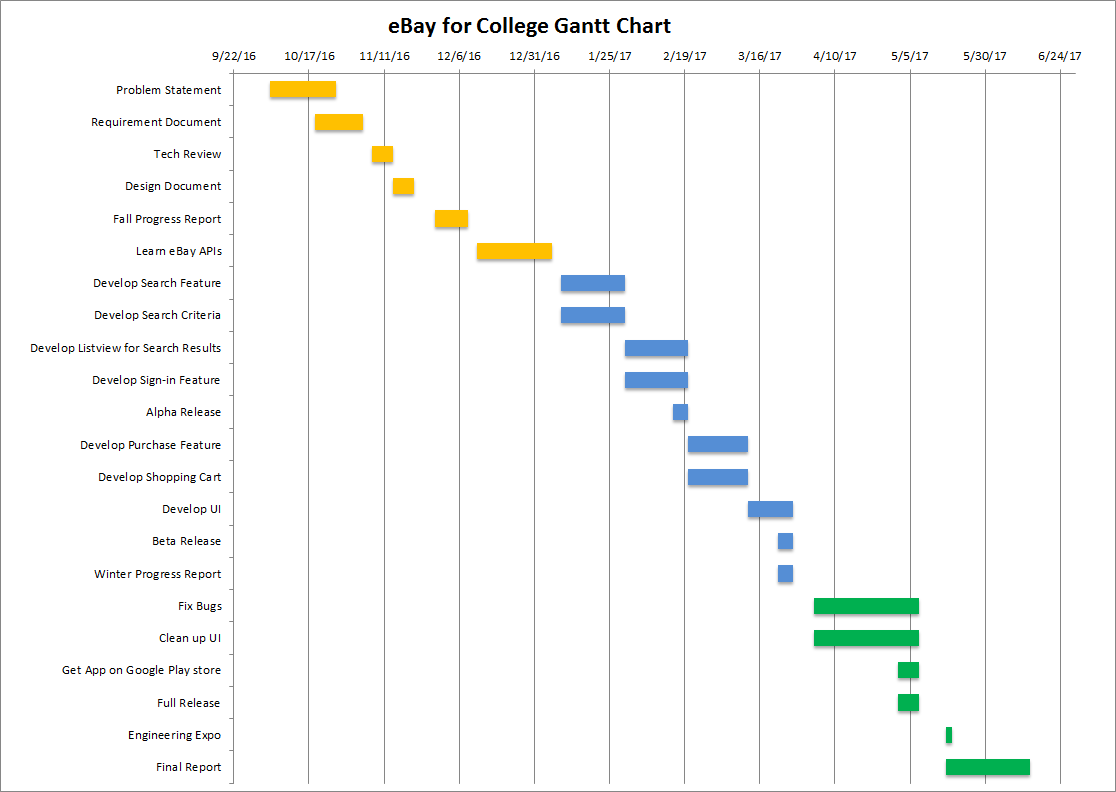
\includegraphics[scale =.6]{ganttChart} 
\centering
\end{figure}

\end{document}